

\section{Boucles et répétitions}
\subsection{Introduction : Un peu de mouvement}

\begin{center}
    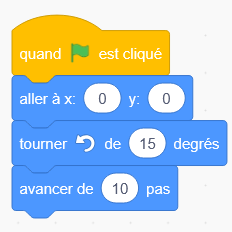
\includegraphics[height=.2\textheight]{tourner.png}
\end{center}
\begin{UPSTIManipulation}{Ajouter du mouvement}
\begin{itemize}
\item Copier le code ci-dessus.
\item Cliquez sur le drapeau vert pour exécuter votre programme. Vous devriez voir le sprite se déplacer et tourner.
\item Cliquer autant de fois que vous voulez pour faire faire un tour complet à votre sprite.
\end{itemize}
\end{UPSTIManipulation}

\UPSTIquestion{Combien de fois faut-il cliquer pour faire un tour complet ?}
\UPSTIquestion{Comment faire pour que le sprite fasse un tour complet sans avoir à cliquer 24 fois ?}


\pagebreak

\subsection{Boucles}
\begin{UPSTIinfor}{Qu'est-ce qu'une boucle ?}
    \vspace{1em}
\textbf{Une boucle est une structure de programmation qui permet de répéter un bloc de code plusieurs fois sans avoir à le réécrire. }\\\\
Par exemple, si vous voulez faire tourner un sprite de 15 degrés 24 fois, vous pouvez utiliser une boucle pour éviter de répéter le bloc "tourner de 15 degrés" 24 fois.
\end{UPSTIinfor}

Sur Scratch, on utilise le bloc "répéter [nombre] fois" pour créer une boucle.

\begin{UPSTIManipulation}{Utiliser une boucle}
\begin{itemize}
\item Ajoutez un bloc "répéter 24 fois" autour des blocs "tourner de 15 degrés" et "avancer de 10 pas".
\item Cliquez sur le drapeau vert pour exécuter votre programme. Vous devriez voir le sprite faire un tour complet en 24 étapes.
\item Modifier le programme pour que le sprite fasse deux tours complets.
\end{itemize}
\end{UPSTIManipulation}

\subsection{Boucles infinies}
\begin{UPSTIinfor}{Qu'est-ce qu'une boucle infinie ?}
Une boucle infinie est une boucle qui ne s'arrête jamais.

Par exemple, si vous utilisez le bloc "répéter indéfiniment", le programme continuera à exécuter le bloc de code à l'intérieur de la boucle sans jamais s'arrêter.
\end{UPSTIinfor}

\subsubsection{Déplacer un sprite au clavier}

\begin{UPSTIManipulation}{Déplacer un sprite au clavier}
    \begin{center}
        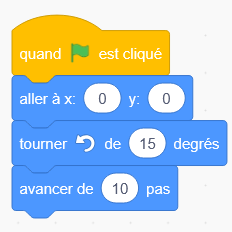
\includegraphics[height=.2\textheight]{deplacer-0.png}
    \end{center}
\begin{itemize}[label=$\square$]
    \item Copier le code ci-dessus.
\end{itemize}
\end{UPSTIManipulation}

\UPSTIquestion{Que se passe-t-il si vous appuyez sur la touche "flèche droite" ?}

\begin{UPSTIidee}{{Pourquoi ?}}
Lorsque le programme est lancé, il vérifie si la touche "flèche droite" est pressée. Si c'est le cas, il déplace le sprite de 10 pas vers la droite. Sinon, il ne fait rien.

Le problème est que le programme ne vérifie pas en continu si la touche "flèche droite" est pressée. Il ne le fait qu'une seule fois au début du programme.

Vous pouvez le vérifier en maintenant la touche "flèche droite" pendant que vous lancez le programme. Le sprite se déplace car la touche est pressée au moment du lancement du programme. Il ne le fait qu'une seule fois, et ne continue pas à vérifier si la touche est pressée.
\end{UPSTIidee}

\begin{UPSTIManipulation}{Corriger le programme}
\begin{itemize}[label=$\square$]
\item Entourez le bloc "si [touche flèche droite pressée] alors" avec un bloc "répéter indéfiniment".
\item Cliquez sur le drapeau vert pour exécuter votre programme. Vous devriez maintenant pouvoir déplacer le sprite en maintenant la touche "flèche droite" enfoncée.
\item Ajoutez des blocs similaires pour les touches "flèche gauche", "flèche haut" et "flèche bas" pour déplacer le sprite dans toutes les directions.
\item \textbf{ASTUCE} : Vous pouvez dupliquer tout le bloc "si [touche flèche pressée] alors" avec un clic droit et en sélectionnant "Dupliquer". Cela vous permettra de gagner du temps pour créer les autres directions.
\item Cliquez sur le drapeau vert pour exécuter votre programme. Vous devriez maintenant pouvoir déplacer le sprite dans toutes les directions en utilisant les touches fléchées.
\end{itemize}
\end{UPSTIManipulation}

\subsubsection{Un premier jeu}

Nous allons ajouter un second sprite qu'il faudra attraper. 

\begin{UPSTIinfor}{Un code pour chaque sprite}
Chaque sprite peut avoir son propre code. Vous pouvez ajouter un nouveau sprite en cliquant sur le bouton "Choisir un sprite" en bas à droite de l'interface. 
Chaque sprite peut avoir son propre code, ce qui permet de créer des interactions entre les sprites.
\end{UPSTIinfor}

\begin{UPSTIManipulation}{Attraper le sprite}
\begin{itemize}
\item Ajoutez un nouveau sprite (par exemple, un chat) à votre projet
\end{itemize}
\textbf{Dans le code de ce nouveau sprite :}
\begin{itemize}
\item Ajoutez un bloc "quand le drapeau vert est cliqué"
\item Ajoutez un bloc "Aller à position aléatoire" pour que le sprite apparaisse à une position aléatoire sur la scène.
\item Ajoutez un bloc "répéter indéfiniment" à l'intérieur duquel vous ajouterez un bloc si touche [votre sprite] alors aller à une position aléatoire.
\item Testez votre programme et faites valider votre programme par l'enseignant.
\end{itemize}
\end{UPSTIManipulation}